\subsection{Conservative Velocity Interpolation (CVI)}\label{sec:CVI}
The CVI correction is checked by means of the Stokes flow experiment by \citet{Donea2003}, as presented in \ref{sec:stokes}. The advection of Lagrangian
markers is performed using either a 2nd-order or a 4th-order Runge-Kutta scheme with CFL=0.5 and an initial random distribution of 25 markers per element.
Fig. \ref{fig:CVI} shows the minimum and maximum values of markers per element throughout the experiment with and without the CVI correction and using
different Runge-Kutta schemes.
The introduction of the CVI correction allows the
tests to run for times longer than $t=2000$ without show empty elements, while tests without the CVI correction stop at approximately $t=600$, when at least
one element goes empty. Fig. \ref{fig:CVI_time} shows the different number of markers per element and the markers distribution at $t=600$ obtained without and
with the CVI correction (panels b and c, respectively) in case of a 2nd-order Runge-Kutta scheme. All data can be found at
\url{https://github.com/aleregorda/Benchmarks/tree/main/Advection/CVI}.
\begin{figure}[h!]
\centering
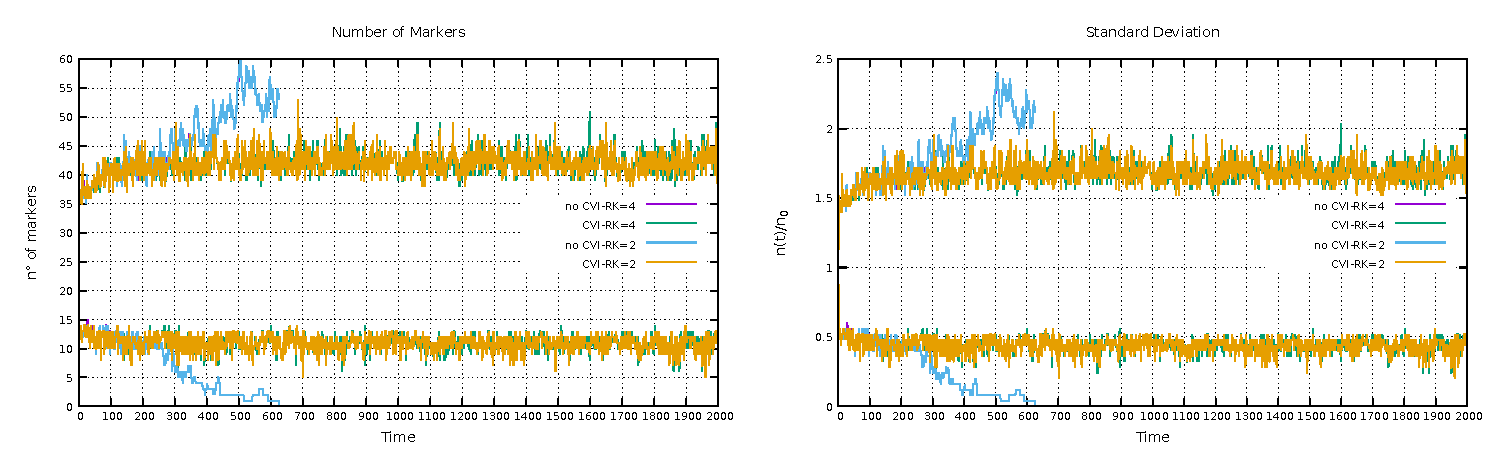
\includegraphics[width=13.5cm]{./Figures/CVI.pdf}
\caption{Maximum and minimum number of markers per element throughout the experiment, with (green and orange lines) or without (purple and blue lines)
the CVI correction and using either a 2nd-order (blue and orange lines) or a 4th-order (purple and green lines) Runge-Kutta scheme.}
\label{fig:CVI}
\end{figure}
\begin{figure}[h!]
\centering
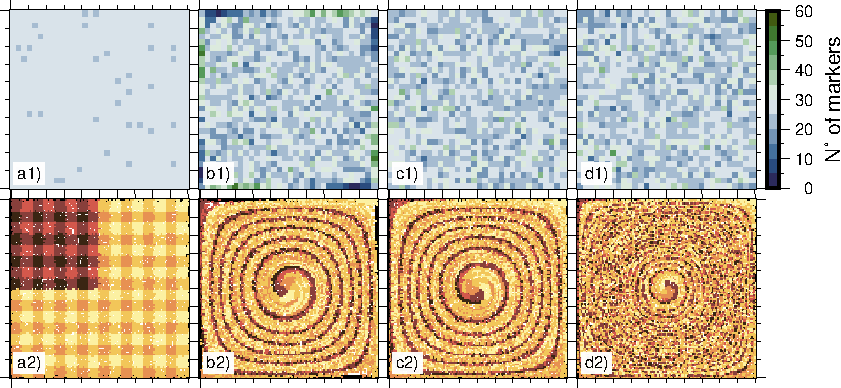
\includegraphics[width=15cm]{./Figures/CVI_time.pdf}
\caption{Number of markers per element and markers distribution through time using 2nd-order Runge-Kutta scheme.
Panels a: number of markers per element (panel a1) and distribution of the markers (panel a2) after the first
iteration; panels b and c: comparison between number of markers per element (panels b1 and c1) and markers distribution (panels b2 and c2) without and with
the CVI correction at $t=600$; panels d: number of markers per element (panel d1) and markers distribution (panel d2) in case of CVI correction at $t=2000$.}
\label{fig:CVI_time}
\end{figure}